\section{Introduction}
\label{sec:intro}
Question motivated dialogues are very common in daily life and 
they are rich sources of question-answer (QA) pairs. 
For example, in an online forum for health consultations, 
both the doctor and the patient tend to ask and answer questions to 
narrow down the information gap and reach the final diagnosis or 
recommendations. Matching QA pairs from such resources is a valuable task. 

QA matching is an important part of analyzing discourse structures 
for dialogue comprehension. Asher et. al~\shortcite{asher2016discourse} 
shows that in online dialogues where participants are prompted to 
communicate with others to achieve their goals, 24.1\% of the relations 
between elementary discourse units are QA pairs. 
Questions and answers are also considerable components of 
dialogue acts~\cite{stolcke2000dialogue}, which are key features for 
doing dialogue summarization and 
decision detection~\cite{fernandez2008modelling}. 
Besides, figuring out the QA relations between these utterances can 
provide question answering 
models~\cite{ji2014information,vinyals2015neural,cui2017superagent} with 
high-quality QA pairs and contribute to the exploration of proactive questioning \cite{yan2017building}.

\begin{figure}[t]
	\centering
	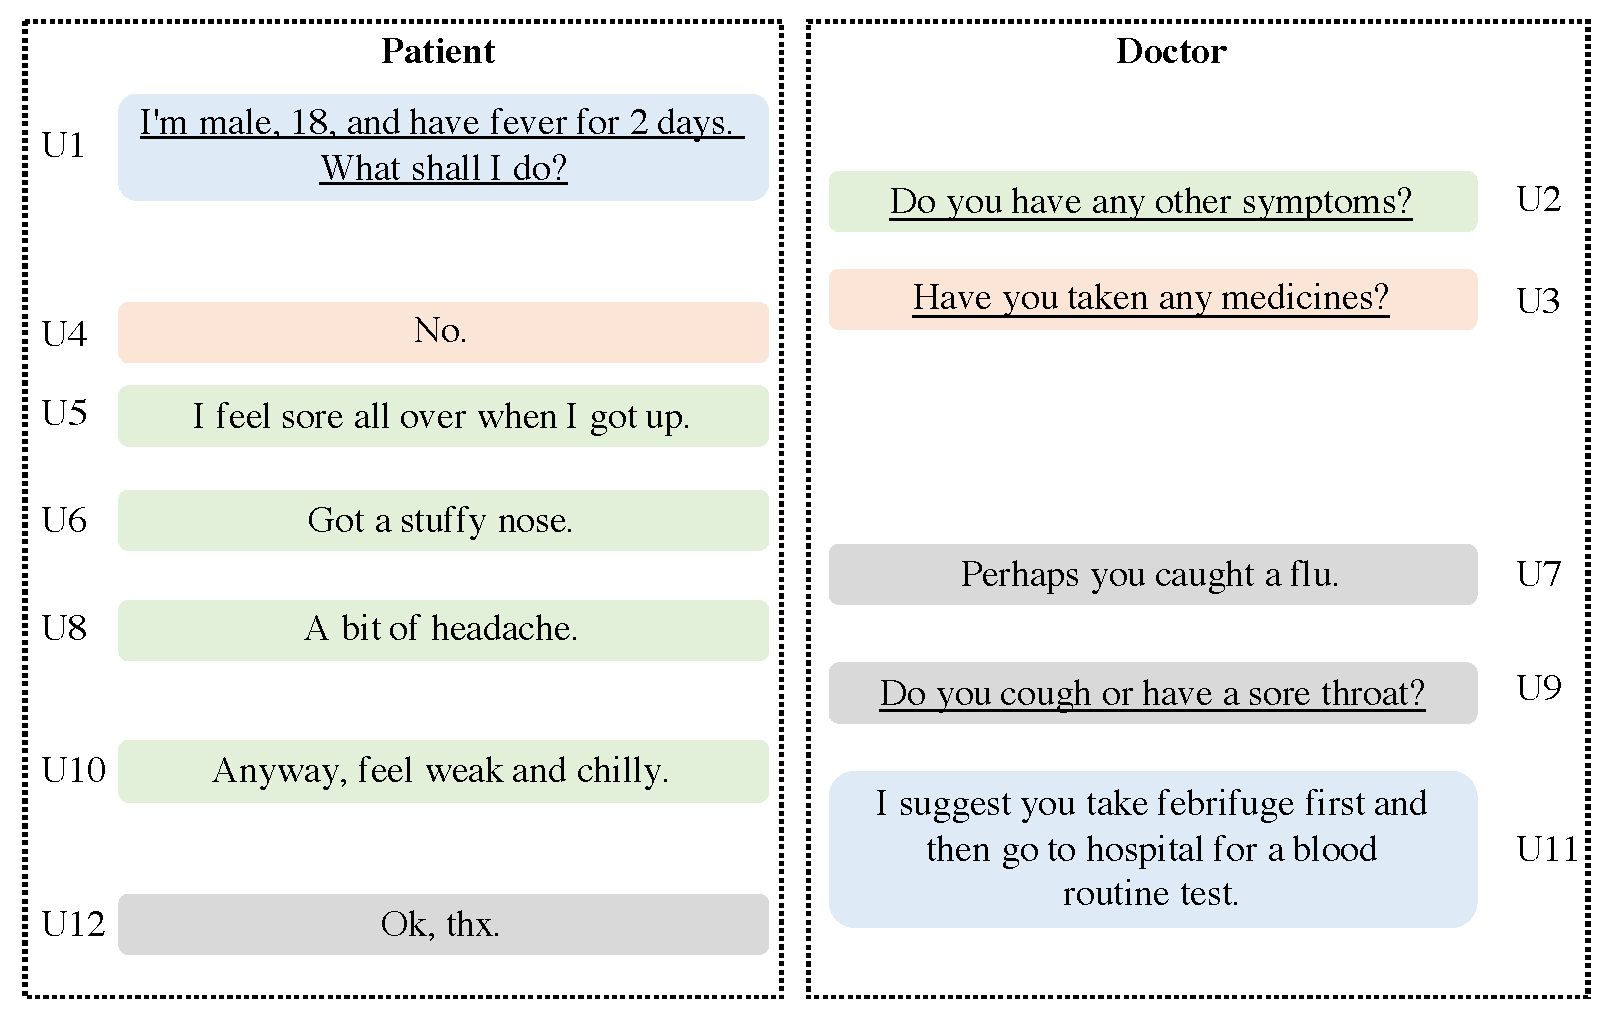
\includegraphics[scale=0.28]{pictures/figure3.eps}
	\caption{Questions and answers matching in dialogues from an online health forum. The identified pairs are painted in the same color and questions are underlined.}
	\label{fig:sample}
\end{figure}

However, many challenges exist. Besides questions and answers, a dialogue also contains chit-chats, distinguished from real answers and informative statements. It is also a common phenomenon that a long and complete answer is broken up into several turns such as \{U5,U6,U8,U10\} in \figref{fig:sample}. Due to factors such as the network delay and differences in typing speed, the dialogue sequences are always mix-matched. Moreover,``personalized" orthography, ellipses, abbreviations, and missing punctuations are all difficulties for QA matching.



In this work, we focus on the task of matching questions and answers in two-party multi-turn dialogues. We found that the distance between the question and its answers isn't only influenced by the mix-matching and fragmentation mentioned above, but also affected by its nature. Some questions can be answered directly based on personal knowledge, such as U3, while others can not. For instance, when a patient asks questions such as ``what's wrong with me'' or ``what should I do'' just like U1, the doctor often has to ask follow-up questions \{U2,U3\} to seek for additional information in order to give the final diagnosis or recommendation (U11) after several turns of communications. We call this kind of QA pairs as {\em incremental QA}. Such QA pairs reflect the main idea of dialogues or sub-dialogues, significantly important for dialogue comprehension. Unfortunately, the answers are inherently far from the question for incremental QA pairs (distance $\geq$ 3 \footnote{There is at least one follow-up question and one corresponding answer between the question and answer of an incremental QA pair. So the distance for such QA pairs is larger or equal to 3.}), aggravating the difficulty of matching such pairs. 

Roughly, we can categorize the QA pairs according to the distance between them. 
When the distance is less than 3, we call it short-distance QA pairs (SQA); 
otherwise, long-distance QA pairs (LQA). 
It is obvious that matching LQAs is much difficult than SQAs. 
We assume that a two-party multi-turn dialogue contains two types of turns, 
questions (Q) and non-questions (NQ), 
which are labeled in advance~\footnote{In practice, automatic utterance labeling with Q and NQ can be done with a simple neural-based classifier, 
which will be released to the research community, 
and its accuracy is more than 96\%.}. 
Our task is to identify all answers from the set of NQs to a given Q. 

Previous methods on the task~\cite{ding2008using,du2017discovering,jiang2018learning} suffer from a major weaknesses: while classifying a pair of turns, they ignore the context of the turns in the dialogue. Meanwhile, their pre-defined features such as question words and answer words, are already implied by the Q and NQ labels in our definition and hence are not suitable for our task. He et al.~\shortcite{he2019learning} improves the above methods with a recurrent pointer network (RPN) model that takes the whole dialogue as an input sample. Their model was evaluated on a closed-source customer service dialogue dataset. Although their model makes use of the context, they treat every utterance in the context equally with RNN-based networks which fails to capture the influences between turns especially with long distance. Besides, it encodes the distance information implicitly which downplays the effect of distance between the utterances. According our experiments, none of the above approaches perform well on LQA pairs.


In this paper, we bring the dialogue context into the simple pairwise model. For a given pair of Q and NQ to be matched, the context is defined as {\em history}, refering to the utterances between the Q and NQ. The critical part of our model is two simultaneous attention mechanisms that combine the history in a mutual way. Compared with the state-of-the-arts and controlled baselines, our proposed models increase the F1-score from 70.46\% to 77.43\% for overall performance. The F1-score for LQAs is 40.44\% and 24.80\% when distance is 4 and $\geq 5$ respectively.

In brief, our main contributions are as follows:
\begin{itemize}
%    \item We focus on the task of matching questions and answers in two-party multi-turn dialogues, and we are the first to category QA pairs based on its distance to the best of our knowledge. (\secref{sec:problem})
    %the fragmentation phenomenon of answers and Complex QA relations which. 
    %It is meaningful for constructing question answering systems, figuring proactive questioning and doing dialog summarization.
    \item We bring dialogue history and distance information into basic pairwise models. We show that distance is an important feature which is suggested to be encoded explicitly. History between Q and A can be effectively captured by a mutual attention mechanism. (\secref{sec:method}) %Based on Q-NQ labels, our approach can match non-questions to questions from both participants and solve different alignment situations in a unified manner 
    % which suggest to be encoded explicitly
    \item Since there is no open source dialogue datasets designed for
QA matching task, especially including long-distance QAs, 
we construct a dataset from online health counselling dialogues,
and will release this dataset to the research community (\secref{sec:data}). 
    \item The experimental results show that our proposed method outperform 
other strong baselines on this dataset, especially on LQAs 
(\secref{sec:results}). The techniques developed here are generic and can
be applied to other kind of online discussion dialogues.
    %Based on proposed approach, we automatically label QA relations for around 160,000 raw dialogues crawled online. Both
\end{itemize}

% The rest of this paper is organized as follows: The next section give a detailed description about the task, the dataset and challenges. Section \ref{sec:method} presentes the proposed technique for the pairwise alignment model. We evaluate our approach in Section \ref{sec:eval}. Section \ref{sec:relatedwork} discuss the related work and Section \ref{sec:conclusion} concludes this paper.
